\documentclass[a4paper,fontsize=10pt,twoside,DIV15,BCOR12mm,headinclude=true,footinclude=false,pagesize,bibtotoc]{scrbook}

\usepackage[utf8]{inputenc}
\usepackage[T1]{fontenc}

\usepackage{pslatex} % -- times instead of computer modern
\usepackage[scaled=.84]{beramono} % a sane monospace font
\usepackage{microtype}

\usepackage{url}
\usepackage{booktabs}
\usepackage{graphicx}
\usepackage{textcomp}
\usepackage{xspace}
\usepackage[usenames,dvipsnames]{xcolor}
\usepackage{colortbl}
\usepackage{multicol}
\usepackage{rotating}
\usepackage{subfig}
\usepackage{ulem}
\usepackage{enumerate}

% avoid clubs and widows
\clubpenalty=10000
\widowpenalty=10000

% tweak float placement
%% \renewcommand{\textfraction}{.15}
\renewcommand{\topfraction}{.75}
%% \renewcommand{\bottomfraction}{.7}
\renewcommand{\floatpagefraction}{.75}
%% \renewcommand{\dbltopfraction}{.66}
%% \renewcommand{\dblfloatpagefraction}{.66}
\setcounter{topnumber}{4}
%% \setcounter{bottomnumber}{4}
%% \setcounter{totalnumber}{16}
%% \setcounter{dbltopnumber}{4}
	
\newcommand{\code}[1]{{\texttt{#1}}}
\newcommand{\codefoot}[1]{{\textsf{#1}}}
\def\figref#1{Figure~\ref{fig:#1}}

% ulem package, otherwise emphasized text becomes underlined
\normalem


\newcommand{\todo}[1]{{\emph{TODO: #1}}}
%\renewcommand{\todo}[1]{}

%
% generic command to comment something
%
\newcommand{\comment}[3]{

\textsf{\textbf{#1}} {\color{#3}#2}}

%
% commentators
%
\newcommand{\tommy}[1]{\comment{Tommy}{#1}{Red}}
\newcommand{\wolf}[1]{\comment{Wolfgang}{#1}{OliveGreen}}
\newcommand{\martin}[1]{\comment{Martin}{#1}{Blue}}
\newcommand{\stefan}[1]{\comment{Stefan}{#1}{RoyalPurple}}
\newcommand{\daniel}[1]{\comment{Daniel}{#1}{RoyalBlue}}
\newcommand{\cullmann}[1]{\comment{Christoph}{#1}{Maroon}}
\newcommand{\gebhard}[1]{\comment{Gernot}{#1}{RedOrange}}
\newcommand{\fb}[1]{\comment{Florian}{#1}{Emerald}}
\newcommand{\jack}[1]{\comment{Jack}{#1}{Magenta}}
\newcommand{\sahar}[1]{\comment{Sahar}{#1}{Green}}
\newcommand{\rasmus}[1]{\comment{Rasmus}{#1}{Mahogany}}
\newcommand{\eva}[1]{\comment{Evangelia}{#1}{Green}}

% uncomment to get rid of comments
%\renewcommand{\tommy}[1]{}
%\renewcommand{\wolf}[1]{}
%\renewcommand{\martin}[1]{}
%\renewcommand{\stefan}[1]{}
%\renewcommand{\daniel}[1]{}
%\renewcommand{\cullmann}[1]{}
%\renewcommand{\gebhard}[1]{}
%\renewcommand{\fb}[1]{}
%\renewcommand{\jack}[1]{}
%\renewcommand{\sahar}[1]{}
%\renewcommand{\rasmus}[1]{}

%
% custom colors
%
\definecolor{lightgray}{gray}{0.8}
\definecolor{gray}{gray}{0.5}

\usepackage{listings}

% general style for listings
\lstset{basicstyle=\ttfamily,language=C}

%\usepackage[endianness=big]{bytefield}
\usepackage{bytefield}

% long immediate in second slot
\newcommand{\lconst}{\texttt{const}_{32}}
% short immediate in ALU instruction
\newcommand{\sconst}{\texttt{Constant}_{12}}
% constant in Rs2 field
\newcommand{\rconst}{\texttt{Constant}_{5}}

% SH: to be used in text mode .. maybe we should change this to math mode?
\newcommand{\XOR}{\textasciicircum\xspace}
\newcommand{\OR}{\textbar\xspace}
\newcommand{\AND}{\&\xspace}
\newcommand{\NOT}{\texttildelow}
\newcommand{\shl}{\textless$\!$\textless\xspace}
\newcommand{\shr}{\textgreater$\!$\textgreater$\!$\textgreater\xspace}
\newcommand{\ashr}{\textgreater$\!$\textgreater\xspace}

\newcommand{\bitsunused}{\rule{\width}{\height}}
\newcommand{\bitssubclass}{\color{lightgray}\rule{\width}{\height}}

%
% allow click-able links
%
\usepackage[open]{bookmark}
\usepackage[all]{hypcap}

%
% hyperref setup (depends on bookmark/hyperref}
%
\hypersetup{
    pdftitle = {Argo programming guide},
    pdfsubject = {Technical Report},
    colorlinks = {true},
    citecolor = {black},
    filecolor = {black},
    linkcolor = {black},
    urlcolor = {black},
    final
}

%
% document contents
%
\begin{document}

\title{Argo Programming Guide}

\author{Evangelia Kasapaki,  Rasmus Bo S{\o}rensen}

\lowertitleback{Copyright \copyright{} 2014 Technical University of Denmark
  \medskip\\
  \begin{tabular}{lp{.8\textwidth}}
    \raisebox{-12pt}{
\includegraphics[height=18pt]{fig/cc_by_sa}} &
     This work is licensed under a Creative Commons Attribution-ShareAlike
     4.0 International License.
     \url{http://creativecommons.org/licenses/by-sa/4.0/}\\
  \end{tabular}
}

\frontmatter

\maketitle

\chapter{Preface}

This guide describes how the Argo NOC can be programmed through a description of the APIA and code examples.
This document should evolve to be the documentation on writing multicore application for the T-CREST platform.

The most recent version of this guide is contained as LaTeX source in the Patmos repository in directory
\code{patmos/doc/noc} and can be built with \code{make}.

\section*{Acknowledgment}
This work was partially funded under the
European Union's 7th Framework Programme
under grant agreement no. 288008:
Time-predictable Multi-Core Architecture for Embedded
Systems (T-CREST).
And partially funded by:
The Danish Council for Independent Research | Technology and Production Sciences (FTP) 
project (Hard Real-Time Embedded Multiprocessor Platform - RTEMP)

\tableofcontents

\begingroup
\let\cleardoublepage\clearpage
%\listoffigures
%\listoftables
%\lstlistoflistings
\endgroup

\mainmatter


%\chapter{Argo Programming Guide}

\chapter{Introduction}

%\section{Introduction}

Argo is a time-predictable Network-on-Chip (NOC) designed to be used in hard real-time multi-core platforms.
The main functionality of Argo is to provide time-predictable core-to-core communication in the form of message passing.
Argo provides time-predictable message passing using Virtual Circuits. Virtual Circuits (point-to-point communication channels)
are implemented using time-division-multiplexing (TDM). According to TDM,
shared resources are allocated to Virtual Circuits based on a static TDM schedule.
The static TDM schedule can be constructed to fit an application requirements by allocating
different amounts of bandwidth to different communication channels.


%The current report assumes that the reader is familiar with C and has skimmed
%through the \href{http://patmos.compute.dtu.dk/patmos_handbook.pdf}{Patmos Handbook} \cite{patmos-handbook}
%on how to build a Patmos processor and Patmos tools.

%The current Argo Programming Guide contains a short description of the Argo architecture in Section~\ref{sec:arch}.
%and a short description of the TDM scheduling in Section~\ref{sec:poseidon}.
%Section~\ref{sec:mem} describes the address space and interface of Argo.
%Chapter~\ref{chap:program} guides the programmer application on how to program an application using Argo 
%(application programming level).

%The Poseidon scheduler available at \url{https://github.com/t-crest/poseidon.git} is part of
%the T-CREST tool chain and is used to generate static TDM schedules.

The steps to build the Patmos tools on a Linux/Ubuntu
system are presented in the \href{http://patmos.compute.dtu.dk/patmos_handbook.pdf}{Patmos Handbook} 
\cite{patmos-handbook}.
In this report we assume that the reader is familiar with C and has skimmed
through the \href{http://patmos.compute.dtu.dk/patmos_handbook.pdf}{Patmos Handbook}.
%Another assumption is the the reader already has access to a hardware platform,
%either genereated by the reader or a pre-synthesized platform downloaded from the project webpage.




\section{The Architecture of Argo}
\label{sec:arch}


\begin{figure}
\centering
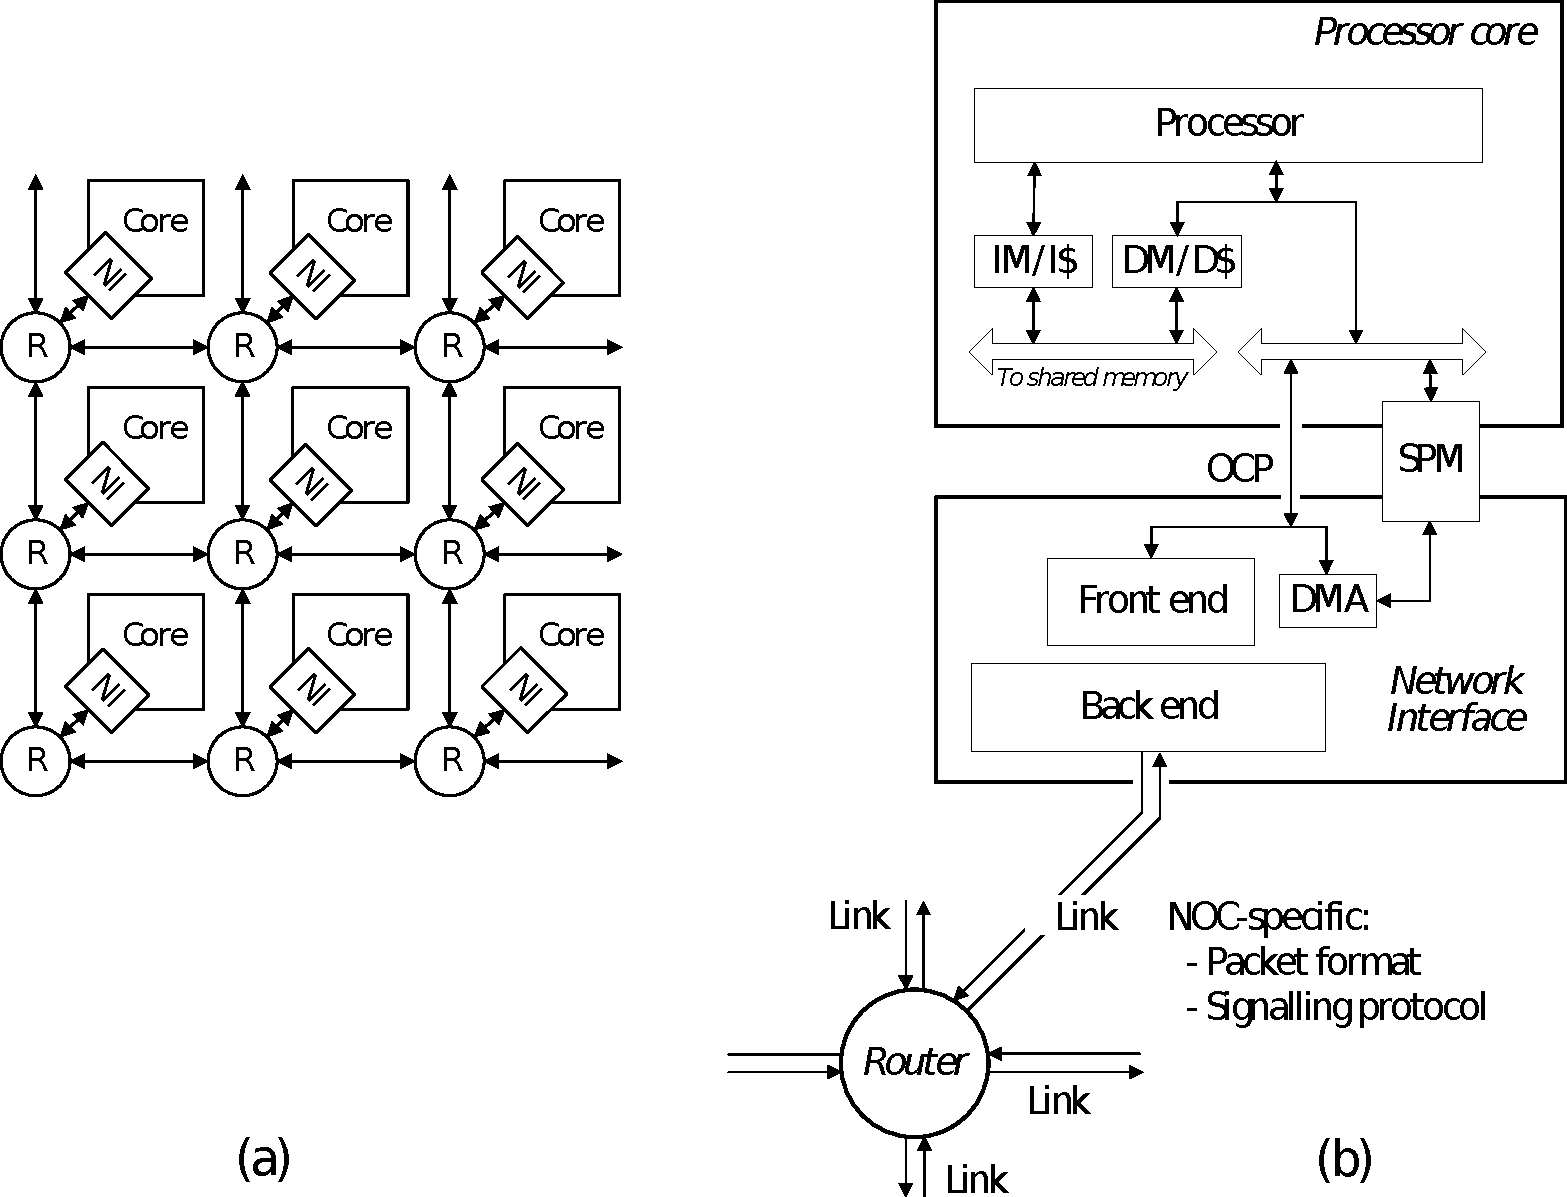
\includegraphics[scale=0.45]{fig/argo.pdf}
\caption{The architecture of a single Argo tile.}
\label{fig:diag}
\end{figure}

The Argo NOC is made up of two different components,
network interfaces (NI) and routers.
The NI converts the transaction based communication from the processor core to
stream based communication towards other processor cores in the network.
The router is routing the stream of packets that are injected from the NIs
through the network according to the static TDM schedule.
The routers are connected in a 2D bi-torus structure.
A diagram of the architecture of Argo is shown in Figure~\ref{fig:diag}(a).


The communication that goes through the network is controlled by the TDM schedule.
A direct memory access (DMA) that is placed in the NI, as seen in Figure~\ref{fig:diag}(b),
is controlling the communication from that NI, enforcing the TDM schedule.
There is one DMA controller per communication channel.
The TDM schedule divides time in time-slots and during one time-slot one 
communication channel, i.e. one DMA, is active.

The NI of Argo has two OCP \cite{ocp:spec} interfaces. The first is a 32-bit interface,
connected to the processor core for configuring of TDM schedule and DMA controllers.
The second is 64-bit interface, connected to the local memory of the processor, i.e. scratchpad memory (SPM),
for accessing the data. The DMA and the SPM of each processor are mapped in the local address space and
can be accessed by the processor through specific load and store instructions.
The exact address space can be found in \cite{patmos-handbook}.
The DMA is setup by the processor core to initiate a message transmission,
creating a direct connection from the local SPM of one processor to the local SPM of a remote processor. 

Details of the architecture and implementation of the NI can be found in \cite{tdmna}.
More details on the router design and the timing characteristics of the NOC can be found in
\cite{noc-elasticity}.



\section{Static Time Division Multiplexing Scheduler}
\label{sec:poseidon}

%The TDM scheduler used to generate schedules for Argo is called Poseidon.
%The source of Poseidon is placed at \url{https://github.com/t-crest/poseidon.git}.
%The performance of Poseidon is desrcibed in \cite{tcrest:poseidon}.% Technical report on poseidon
%
%Poseidon takes an XML file as input descriping the platform and the required communication pattern.
%The platform and communication tags can be given in two different XML files or on one.
%When the platform is generated from the Aegean platform generator, the input files for the scheduler are also generated.
%
%For the time beeing the scheduler is limited to schedule one package per communication channel in each period.
%This limitation is due to a limitation in the current hardware, not a limitation in the scheduler it self.
%When multiple packages per communication channel are supported the limitation can be removed by commenting out (in t-crest/poseidon/src/parser.cpp) the lines:
%
%\begin{verbatim}
%warn_if(bw != 1,"Bandwidth different from 1 is not supported by Argo, Bandwidth set to 1.");
%if (bw != 1) { bw = 1;  }
%\end{verbatim}

%\subsection{Input format}

%\subsection{Output format}

%\subsection{Conversion to C}

The TDM scheduler used to generate schedules for Argo is called Poseidon.
The source of Poseidon is placed at \url{https://github.com/t-crest/poseidon.git} and
it is described in \cite{scheduler-report}.

\begin{figure}
\centering
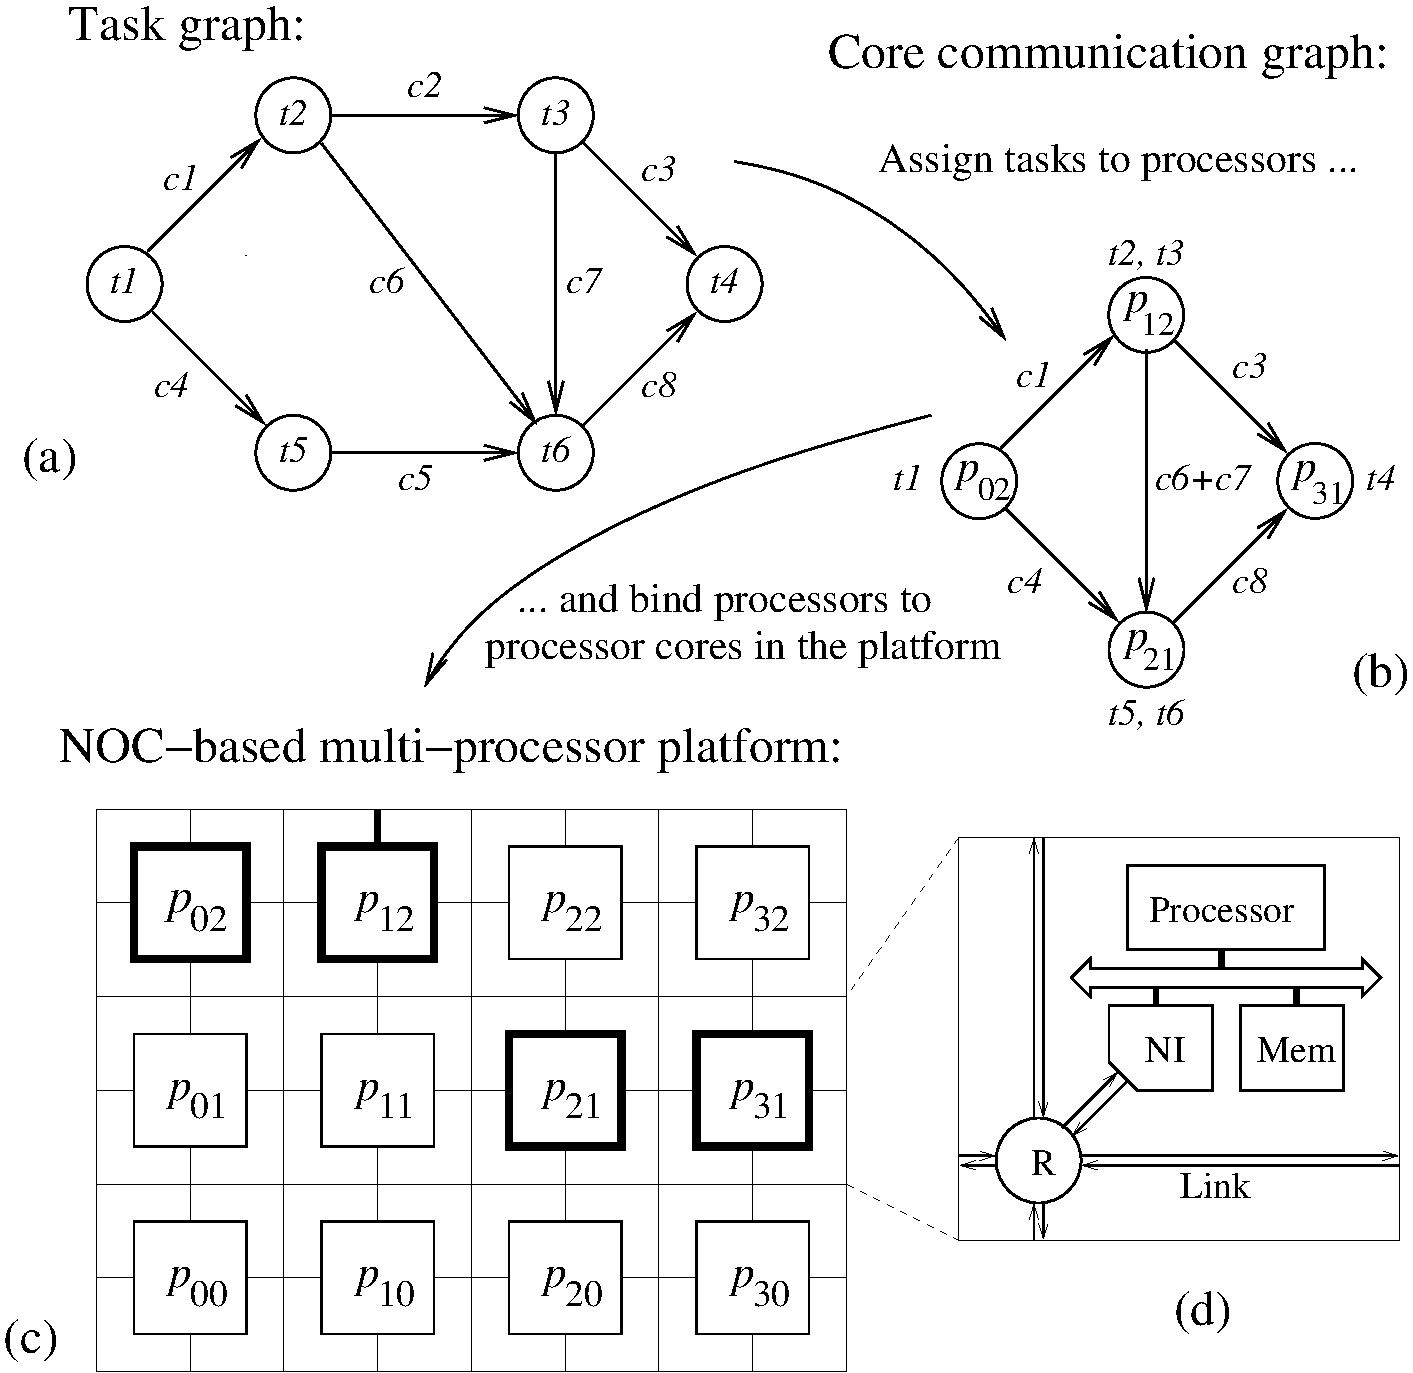
\includegraphics[scale=0.4]{fig/flow.pdf}
\caption{ Mapping of an application onto a multi-processor platform: (a) Task graph for application, (b) core communication graph, 
(c) multi-processor platform, and (d) details of a node in the platform (router (R), links, network interface (NI), processor and local memory).}
\label{fig:flow}
\end{figure}


The scheduler is mapping an application onto an application-independent multi-processor platform with the following steps, as illustrated in Figure~\ref{fig:flow}.
An application is modeled as a {\em  task graph} where nodes represent tasks and edges represent communication channels (end-to-end circuits).
The first step is to assign tasks to processors and as part of this to decide which tasks will share a processor.
The result of this is a {\em core communication graph} where the nodes represent processors and the edges represent communication flows and their required bandwidth between the processors.
The second step is the binding of processors to specific processor cores in the platform. %This usually aims at minimizing the total number of router-to-router hops for traffic. 
%The first and second steps are not specific for TDM-based NOCs and they are well studied in the literature. Early works include \cite{Murali2004}.
The third step is to generate the TDM schedule for Argo.


\section{Argo Usage}

Argo can be used in three different levels. In the first level (application programing level)
a standard platform and a static predefined schedule are provided. The platform is an NxM platform,% with up to 64 nodes, 
operating on an all-to-all schedule with the same bandwidth assigned to every channel. The details 
on platform initialization, TDM schedule creation and channel configuration are hidden from an
application programmer. Instead, library tools are provided for sending messages from
processing cores to remote processing cores. The current report focuses on this level of usage.

At a second level (task scheduling level) a fixed platform is provided but a different schedule 
can be produced based on the task graph and the communication requirements. The details of the schedule
production are not presented in the current documentation.

At a third level (platform configuration level) the user can configure a different hardware platform.
The configured parameters that can be defined for the platform can be the size of the NOC in an NxM structure,
the connecting topology (bi-torus/mesh) and the sizes of memories used (main memory, SPM, cache).
The details on different platform configurations are not presented in the current documentation.


%The current Argo Programming Guide contains a description of the Argo architecture in Section~\ref{sec:arch}.
%Section~\ref{sec:poseidon} describes how to generate a static TDM schedule.
%Section~\ref{sec:mem} describes the address space and interface of Argo.
%Section~\ref{sec:apg} guides the reader on how to program an application that uses the NOC.


\chapter{Argo Programming Guide}
\label{chap:program}

This chapter refers to the use of Argo on application programing level.

\section{Operation of Argo}
\label{sec:oper}

Argo implements message passing functionality. A processor can push data 
to a remote processor, i.e. a task running on a processor
can send messages to a task running on a remote processor.
Each processor has an SPM that is mapped to its local address space.
The data to be sent should be placed in the SPM of the local processor.
From there the data is sent through a channel in the network and placed in a 
specified address in the remote SPM. 

The sending is controlled by the DMA controller and based on the TDM schedule.
The initialization of the TDM schedule is done automatically through initialization 
of the Aegean platform. The configuration of the DMA is done by the processor.
The details of this operation are hidden from the application. However,
the application programmer is offered a library, \textit{libnoc} library,
with the necessary variables and functions. The full list of variables in libnoc 
can be seen in Section~\ref{sec:apg}.

While the initialization of SPM and configuration of DMA are not transparent to the programmer,
the programmer is responsible for the explicit handling of data and the communication in terms of
source and destination and SPM addresses. 
Thus, the programmer should explicitly place data to an address in the local SPM. 
From each core there is one communication channel to every other core.
A sending function is offered in \textit{libnoc} where the programmer should specify 
the sending channel in terms of destination core as well as the source and destination SPM address. 
The path information and routing through the network as well as details of the sending operation 
are hidden from the programmer.



%Argo is initialized with the initialization of the Aegean platform. Variables such as
%\code{NOC\_CORES} and \code{CORE\_ID} are initialized automatically with the configuration
%of Aegean. The full list of variables in libnoc can be seen in Section~\ref{sec:apg}.


%%\chapter{Memory address space and interface}
%\section{Memory address space and interface}
%\label{sec:mem}
%
%
%The UART and LEDS are also mapped in the local address space and can be accessed only by the master core
%at the specific addresses.
%
%\subsection{Local Address Space}
%
%\begin{description}
%\item[UART\_STATUS]      0xF0000800
%\item[UART\_DATA]        0xF0000804
%\item[LEDS]              0xF0000900
%\item[NOC\_DMA\_BASE]    0xE0000000
%\item[NOC\_DMA\_P\_BASE] 0xE1000000
%\item[NOC\_ST\_BASE]     0xE2000000
%\item[NOC\_SPM\_BASE]    0xE4000000
%\item[NOC\_VALID\_BIT]   0x08000
%\item[NOC\_DONE\_BIT]    0x04000
%\end{description}


%\chapter{Build Instructions}
\section{Build Instructions}

%In the following we present the Patmos build instructions on a Linux/Ubuntu
%system.\footnote{I used the 32-bit version of Ubuntu to simplify the Quartus installation.}
%Patmos and the compiler have also been successfully installed on a Mac OSX
%system. The support of Windows is marginal, or basically not existent.
In the following we present the build instructions on a Linux/Ubuntu system,
for a 2x2 Aegean platform. The default hardware platform includes 4 Patmos processors 
connected by the Argo NOC and memory arbiter giving access to the shared memory.


\subsection{Aegean Platform Build Instructions}

Information on how to build a Patmos processor and how to run the compiler for Patmos and some application examples
can be found in \cite{patmos-handbook}. 

The platform can be checked out from GitHub as part of the T-CREST project.
The T-CREST project will live in \code{\$HOME/t-crest} and the Aegean platform with Argo NOC
can be checked out and build with the same commands as for Patmos and the compiler.%, as follows:

%\begin{verbatim}
%mkdir ~/t-crest
%cd ~/t-crest
%git clone https://github.com/t-crest/patmos-misc.git misc
%./misc/build.sh
%\end{verbatim}


Several packages and tools need to be installed and setup. The list of packages 
and detailed setup instructions can be found in \cite{patmos-handbook}.
Additionally, \cite{patmos-handbook} describes a simple Hello world application 
to be run either by simulation or on FPGA board, for a single Patmos processor.


The whole build process of an Aegean platform,\footnote{Get
the source from GitHub with: \code{git clone git@github.com:t-crest/aegean}}
applications in C, configuration of the FPGA, and downloading an
application is \code{Makefile} based. The build of the platform is
done in the aegean folder, therefore, the following descriptions
assumes you have changed to:
\begin{verbatim}
	t-crest/aegean
\end{verbatim}

The default platform is 4 Patmos cores connected by a 2x2 bi-torus
Argo NOC and a memory arbiter connecting to main memory, with a memory
controller and pin definitions suitable for the Altera DE2-115 board.
The platform is generated by the command:
\begin{verbatim}
make platform
\end{verbatim}

To synthesize the platform for the FPGA board, run:
\begin{verbatim}
make synth
\end{verbatim}

The synthesized platform is configured on the FPGA with the command:
\begin{verbatim}
make config
\end{verbatim}

The configuration can be changed by setting the \code{AEGEAN\_PLATFORM}
variable in the above make command. The currently supported boards are:
\begin{itemize}
\item Altera DE2-115 (\code{default-altde2-115})
\item Altera DE2-70 (\code{default-altde2-70})
\item Xilinx ML605 (\code{ml605\_4core\_oc}, only on-chip memory)
\end{itemize}
More configurations can be found in the directory \code{config}, where
it is also possible to add custom configurations.

\subsection{Applications}

Applications for the multicore platform can be developed in C code, either 
compiled with the hardware platform, and synthesized on the the on-chip ROM of the FPGA
or compiled in ELF binaries, and booted by a bootloader application on FPGA.
The bootloader is compiled and synthesized as the default application 
along with the platform when \code{make synth} is run.


The application is written in C and should be placed under /t-crest/patmos/c.
In both cases the application is build through \code{Makefile} using the following variables:

\begin{itemize}
\item \code{BOOTAPP} for the built-in on-chip ROM applications.
\item \code{APP} for the ELF binary applications to be executed by the bootloader.
\end{itemize}

%The \code{Makefile} use following variables to configure the build process:
%\code{BOOTAPP} is an application that ends in the on-chip ROM. This may
%be an assembler program or a simple C program;
%most prominent the boot loader for ELF binaries.
%A C program that shall be compiled as ROM target needs to be prefixed
%with \code{bootable-}.
%\code{APP} is a C program resulting in an ELF binary that can be either
%loaded by the emulator or the boot loader when executing in an FPGA.
%% TODO: test and talk about patsim. Having a complete ELF in the FPGA
%% without the boot loader would be nice as well.
%

\subsection{Download of ELF files}

An application executed in the multicore platform can be compiled in an ELF file and downloaded on the FPGA.
The compilation and downloading is make-based and is done in folder /t-crest/patmos/ with the following make commands:

\begin{verbatim}
make APP=<app_name> comp
make APP=<app_name> download
\end{verbatim}

For a new application the corresponding dependencies should be added in the Makefile that
lies under /t-crest/patmos/c.



%\chapter{Application Programming Guide}
\section{Application Programming Guide}
\label{sec:apg}

\subsection{Application Programming Interface}

Library libnoc is providing an application programming interface. A number of functions and variables are provided through libnoc library. 
and they are used for two different purposes. The first is to initialize the network interface (NI) and the second is the setup DMA transfers 
for sending messages to other processing cores. The variables and the functions defined in libnoc are set automatically by the initialization process 
of the Aegean platform and only a subset of them are used by the application programmer. The complete list is presented in the following for reference
purposes.


\subsubsection{Variables:}
\begin{description}
\item[NOC\_CORES] The number of cores on the platform. 
\item[NOC\_TABLES] The number of tables for the NOC configuration.
\item[NOC\_TIMESLOTS] The number of timeslots in the TDM schedule. 
\item[NOC\_DMAS]	The number of DMAs in the configuration. 
\item[noc\_init\_array] The array for initialization data. 
\item[NOC\_MASTER] The master core, which governs booting and startup synchronization. 
\end{description}


\subsubsection{Functions:}
\begin{description}
\item [noc\_configure] Configure network interface according to initialization information in noc\_init\_array.
\item [noc\_init] Configure network-on-chip and synchronize all cores. 
\item [noc\_dma] Starts a NoC transfer. 
\item [noc\_send] Transfer data via the NoC. 
\end{description}

\subsubsection{Defines:}
\begin{description}
\item [NOC\_INIT] Define this before including noc.h to force the use of noc\_init as constructor. NOC\_INIT does not need to be defined if any functions from libnoc are used.
\item [NOC\_VALID\_BIT] The flag to mark a DMA entry as valid.
\item [NOC\_DONE\_BIT] The flag to mark a DMA entry as done.
\item [NOC\_DMA\_BASE] The base address for DMA entries.
\item [NOC\_DMA\_P\_BASE] The base address for DMA routing information.
\item [NOC\_ST\_BASE] The base address for the slot table.
\item [NOC\_SPM\_BASE] The base address of the communication SPM.
\end{description}

\subsection{Hello World Multicore}

An application running on the T-CREST multicore platform consists of a main function that is running on all cores.
Each core is assigned a \code{CORE\_ID} through the initialization process. The distribution of the workload is 
decided by the programmer defining a function with the workload for each specific core. The corresponding function
is called through main by checking the \code{CORE\_ID}. In the T-CREST platform one of the cores has the role of the master
which is the only one that has access to IO. Thus, it can be used as the point of synchronizing and collecting overall data,
as well as outputing the data for viewing purposes.

To demonstrate the use of Argo, a multicore Hello World application \textit{hello\_sum.c} is placed in /patmos/c.
The application is written in C and can be compiled and downloaded on the FPGA board.
%An application running on T-CREST multicore platform conists of a main funtion and depending
In \textit{hello\_sum} application, a round trip "hello" message is sent from the master core
passing through all the slave cores. Each core is adding its ID to the sum of the IDs and 
eventually the master will receive the sum of all core IDs.


\subsubsection{Compile and Run}
For any application to be compiled and run, it needs to be placed in /patmos/c and the target and dependencies 
should be added in the Makefile in the same directory.
To compile and download \textit{hello\_sum} application on the board, the following make commands are used:

\begin{verbatim}
make APP=hello_sum comp
make APP=hello_sum download
\end{verbatim}

\subsubsection{SPM Access}
To develop an application that runs on T-CREST platform, data memory and communication should be handled explicitly by the programmer. 
Argo NOC and the TDM schedule are initialized automatically through Aegean platform but the communication should be handled by the application programmer.
An application is provided access to the main memory (shared), to a number of local SPMs as well as to a communication SPM.
In the current report, when SPM is mentioned, it refers to the communication SPM used by Argo NOC.

To send data from one core to another, the sending application should specify an address in the local SPM of the sending core and place the data there.
To receive data from another core, the receiving application should specify an address in the local SPM where the data are expected. Thus, the 
destination address in the receiving SPM should be known by both sending and receiving applications.
The base address of the communication SPM is \code{NOC\_SPM\_BASE} as defined in the libnoc library 
and any address of the SPM can be used for either sending or receiving purposes or even for directly processing data.
Pointers to access SPM space are defined as:

\begin{lstlisting}
volatile _SPM <type> *<name>
\end{lstlisting}

The copying of the message should be done manually, copying one-by-one character or integer.
The platform operates as \textit{bigendian}.
Copying of strings through string.h is not available. 

%Listing~\ref{lst:hello_master} shows the code executed in the master core.
%The code for the explicit copying the data to the SPM space, the sending of message,

\subsubsection{Sending}
A message is sent using function noc\_send():

\begin{lstlisting}
void noc_send (int rcv_id, volatile void _SPM *dst, volatile void _SPM *src, size_t size)
\end{lstlisting}

The function returns when the DMA transmitting the message is setup. \code{rcv\_id}
is the ID of the receiving core, \code{dst} the write address
in the destination SPM, \code{src} the read address
in the source SPM and \code{size} the size of the message to be transferred in bytes.


%The explicit copying of data to the SPM space and the sending of message appears 
%in Listing~\ref{lst:hello_master}. Listing~\ref{lst:hello_master}
%shows the code executed in the master core.

\subsubsection{Receiving}
Currently, libnoc library does not support a receive message function,
therefore a receiver needs to wait and poll in order to know when the data has arrived.
To do so, specified addresses where the data are expected to arrive are defined and
initialized to 0 before every reception of new data. The receiving application is polling this address to
know if the data has arrived or not and needs to clear it after the reception is complete and data are read.
Since data is transmitted in packets, to safely consider the reception of the entire message
completed, the polling should be done on the last unit of data (char/ int/...) of the message sent.

%In the hello\_sum application, master is sending 
%Listing \ref{lst:hello_multi} shows the code executed in the slave cores.
%The code for the allocation of memory in the SPM, the polling and the sending of message 
%appears in Listing \ref{lst:hello_multi}. 

\subsubsection{Printing}
To print a message, functions \code{puts} and \code{printf} can be used. Data can be print only
by the master core and only if it is placed in the main memory of the program. Therefore,
a data value that is placed in the SPM should be copied in an application variable in main-memory
and then print through \code{puts} or \code{printf}. 

%Listing~\ref{lst:hello_master} shows how to print a static string and a message received in SPM through NOC.

%In the code, \begin{verbatim} spm_slave \end{verbatim}
%is the starting addres where the data is expected in the slave cores. 
%\begin{verbatim} spm_slave + 20 \end{verbatim} is the last char expected in the destination.
%Thus, when the last char arrives it is safe to assume that the entire message has arrived.

\begin{lstlisting}[float,caption={A 2x2 Hello World application: Master application.\label{lst:hello_master}}]
volatile _SPM char *spm_base = (volatile _SPM char *) NOC_SPM_BASE;
volatile _SPM char *spm_slave = spm_base + 64;
*(spm_slave+20) = 0;

// message to be send
const char *msg_snd = "Hello slaves sum_id:0";
char msg_rcv[22];

// put message to spm
int i;
for (i = 0; i < 21; i++) {
	*(spm_base+i) = *(msg_snd+i);
}

// send message
noc_send(1, spm_slave, spm_base, 21); //21 bytes

puts("MASTER: message sent: ");
puts(msg_snd);

// wait and poll
while(*(spm_slave+20) == 0) {;}

// received message
puts("MASTER: message received:");
// copy message to static location and print
for (i = 0; i < 21; i++) {
	*(msg_rcv+i) = *(spm_slave+i);
}
*(msg_rcv+i) = '\0';
puts(msg_rcv);

\end{lstlisting}




\begin{lstlisting}[float,caption={A 2x2 Hello World application: Slave application.\label{lst:hello_slave}}]
volatile _SPM char *spm_base = (volatile _SPM char *) NOC_SPM_BASE;
volatile _SPM char *spm_slave = spm_base + 64;

// initialize polling address to 0
*(spm_slave + 20) = 0;

// wait and poll until message arrives
while(*(spm_slave + 20) == 0) {;}

// PROCESSING DATA : add ID to sum_id
*(spm_slave+20) = *(spm_slave+20) + CORE_ID;

// send to next slave
int rcv_id = (CORE_ID==3)? 0 : CORE_ID+1;
noc_send(rcv_id, spm_slave, spm_slave, 21);

\end{lstlisting}

\subsubsection{Master - Slave Application}
The code for the \textit{hello\_sum} is shown in Listing~\ref{lst:hello_master} and ~\ref{lst:hello_slave}, 
for the master application and the slave application respectively.
Master is using \code{spm\_base} address for the data to be sent out, thus is copying the characters of the message one by one to \code{spm\_base}.
Master is using \code{spm\_slave} as a destination address to the slaves, as well as a receiving address for the expected data from the slaves. 
The slaves use \code{spm\_slave} as receiving and sending address of the message. \code{spm\_slave + 20} is the last character of the message, 
thus it is the address to be initialized to 0 and to be polled to detect the completion of the reception for both the master and slaves.

%\chapter{Pending Changes}
%\section{Pending Changes}
%
%This is a live and temporary section that lists pending changes of Argo.
%
%Currently we have following proposals for a change:
%
%\begin{itemize}
%\item DMA read
%\item Generate an interrupt when a complete DMA transfer has been received. 
%\end{itemize}

% % % % % % % % % % % % % % % % % % % % % % % % % % % % % % % % % % % % % % % %
%\chapter{Potential Extensions}
%\section{Potential Extensions}
%\label{chap:ext}
%Ideas for extensions can be added in this chapter.


Matrix multiplier is another application developed for Argo. 
The source can be accessed at: 
\url{https://github.com/t-crest/patmos/blob/master/c/matrix_mult.c}

\bibliographystyle{abbrv}
% MS noc.bib is missing
\bibliography{argobib}

\end{document}

\appendix


\end{document}
